\documentclass[letterpaper,twocolumn,10pt]{article}
\usepackage{url,epsfig}
\begin{document}

% Don't output date
\date{}

% Title
\title{\Large
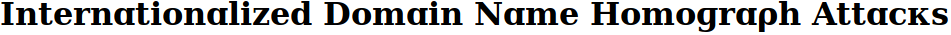
\includegraphics[height=\baselineskip]{title.png}
\\ \vspace{0.65mm} \large \normalfont
CSE 227: Computer Security - Spring 2017 \\ \textit{
University of California San Diego
}}

% Authors
\author{
{\rm Chen Lai}\\
\normalfont{\texttt{chl588@ucsd.edu}}
\and
{\rm Zhongrong Jian}\\
\normalfont{\texttt{zhjian@ucsd.edu}}
\and
{\rm J. Sidrach}\\
\normalfont{\texttt{jsidrach@ucsd.edu}}
}

\maketitle

\abstract{TODO}

\section{Introduction}
Domain names were originally designed to only support ASCII characters.
Internationalized Domain Names (IDNs) were proposed back in December 1996 by Martin D\"{u}rst for the purpose of letting non-English speaking people use Internet without additional restrictions.
This extension involves representing Unicode characters in ASCII using Punycode, so that they could be then rendered back into their Unicode representation.
Homograph letters (different letters whose representation is almost, if not, the same), however, present a potential vulnerability.
For example, Cyrillic letter ``a'' can look identical to Latin letter ``a'' depending on the font.
In other languages, like Chinese, there exists many homograph letters between traditional Chinese and simplified Chinese.
Malicious attackers can then register a domain where one of the letters is actually Cyrillic but whose representation matches a Latin one.
Users could be linked to this newly registered malicious page, and they may not have any visual indication (at least without further interaction) that the page is not the one they think they are visiting.

In this paper, we analyze the impact of this attack.
Section 2 explains past and present policies of major browsers and top level domain registrants in an attempt to prevent the attack.
Section 3 explores relevant work in the literature related to homograph attacks.
Section 4 describes the methodology of data collection and analysis adopted in this project.
Section 5 comments the different results obtained.
Section 6 addresses the ethical concerns regarding the data collection.
Section 7 presents the conclusions obtained from this project.

\section{Background}
TODO
- Browsers policy
- TLDs policy

\section{Related Work}
TODO
- Brief analysis of previous papers on the same topic

Many relevant studies have been conducted to show the vulnerability of IDN and provide possible solution to mitigate IDN homograph attack.
In 2001, Evgeniy Gabrilovich and Alex Gontmakher has proved the feasibility of such attack based on the vulnerability of Unicode in \textit{The Homograph Attack}~\cite{theHomoAttack}.
In 2006, Vicktor Krammer proposed a defense mechanism based on address bar highlighting/indication technique and better UI of the browsers~\cite{phishdefenseKV}.
His method of defense mainly target at regular users who do not necessarily have relevant knowledge and through the better rendering of address along with explicit notification or alert on phishing URL users would be aware of malicious website.
Manurer and Höfer believed that safe guard based on browsers' blacklist is far from enough to protect users from sophisticated phishing attacks~\cite{proc-eds-2012}.
They proposed an advanced method based on URL components and spell checking functionality of search engine.
In this method, an URL would be divided into several components, namely, base name, sub-domains, path domain, brand name.
Each of this components will be sent to search engine as a term for spelling check and in the cases that spelling suggestion is returned the URL will be counted as suspicious.
The major browsers have their own IDN policies to defend against IDN homograph attack.
Google Chrome, starting with Chrome 51, will display Punycode if certain tests fail on the input URL.
These tests include but not limited to converting to Unicode, less than one numbering systems involved, no invisible characters, etc.
IE displays URLs in IDN form if every component contains only characters from the languages configured in \textit{Internet Options}.
Firefox uses a script mixing detection algorithm based on \textit{"Moderately Restrictive" profile of Unicode Technical Report 39} and displays Unicode when URL consists of any single script, any single script plus Latin, or it's in the white-list of other combinations.
Opera shows IDN only for whitelisted TLDs.
Safari has a whitelist of scripts that do not contain confusable characters and only shows the IDN form for the whitelisted scripts.

\section{Methodology}
Our data collection involves two primary sources.
The first one is a snapshot of the \texttt{.com} and \texttt{.net} domain zone, from now on referenced as \textit{.com snapshot}.
This snapshot was provided by Verisign\footnote{\url{https://www.verisign.com/en_US/channel-resources/domain-registry-products/zone-file/index.xhtml}}, and it is dated on 2017/05/01.
It contains, mostly, the name servers of all \texttt{.com} and \texttt{.net} domains.
For the purposes of this project, only the \texttt{.com} domains were considered.

The second data source is the \textit{Alexa Top 1 million sites ranking}\footnote{\url{https://www.alexa.com/topsites}}, from now on referenced as \textit{top domains snapshot}.
It contains the most popular one million web sites, regardless whether they are \texttt{.com} domains or not.
It was also retrieved on 2017/05/01.

In an effort to help with the reproducibility and replicability of this project, the original data and processing code used in this project has been made available in a public repository\footnote{\url{https://github.com/jsidrach/idn-homograph-attack}}.

\subsection{Data Processing}
We used the \textit{.com snapshot} to obtain all the internationalized domains of the \texttt{.com} domain zone.
All internationalized domain names are represented using Punycode, so they start with the \texttt{xn--} prefix.
Using this information we first filtered the \textit{.com snapshot} to match only the \texttt{.com} domains that start with \texttt{xn--}.
Since the \textit{.com snapshot} contains name server records, a single domain may have more than one entry in the file.
Only the domain name is relevant for this project, so the rest of the columns of the \textit{.com snapshot} were discarded.
We sorted the domains in lexicographic order, removing duplicates in the process.

We used the \textit{top domains snapshot} as a source for the canonical (non-international) domain name of a website, based on its ranking.
As we were only interested in non-internationalized domain names, so we discarded the ones that start with the prefix \texttt{xn--}.
We also removed sub-domains, as we only had top level domain names in the \textit{.com snapshot}.

\subsection{Clustering}
The underlying assumptions behind the clustering process are that homograph attacks are more likely to target popular domains, and that the million domains from the \textit{top domains snapshot} contains most of the popular domains.
To detect potential internationalized domain name homograph attacks, we cluster the internationalized domain names in the \textit{.com snapshot}.
The representative of each cluster is a homograph domain name from the \textit{top domains snapshot}.
Only clusters with more than one domain name are output.

The detection of homograph domain names is done using an algorithm to check if two strings are confusable.
This algorithm is described in the \textit{Unicode Technical Standard \#39}\footnote{\url{http://www.unicode.org/reports/tr39/#Confusable_Detection}}.
The approach followed has some caveats, that could be addressed in future work.
For instance, it does not detect a homograph of \texttt{www.google.com}, where the first ``.'' has been replaced by a similar looking Unicode character.
More sophisticated homographs can also be generated by using Unicode characters similar to ``/''.
It is also worth noting that only domain names from the \texttt{.com} zone were considered, but similar studies could be done to other top level domains following the same procedure.
All things considered, we still think this approach is a valuable first step.

Another type of clustering was also performed.
We grouped the homograph domain names by its registrant organization, and ranked each organization by the number of homograph domain names to their name.
This could shed light on which registrant organizations are allowing homograph domain names, or even on which individuals and companies are doing it the most.

\subsection{Manual Classification}
The last part of the data processing was the classification of the homograph domain names.
This classification was done manually, to be able to differentiate between scam and unrelated websites.
To help with the classification and speed up the process, we queried the \textit{WHOIS} records~\footnote{\url{https://whois.icann.org}} of every homograph domain name.
Some domains expired at the time of the classification, and were subsequently deleted from the output file.

The two high level categories that were defined are \textit{Canonical} and \textit{Third Party}.
The first one, \textit{Canonical}, is employed when the domain is registered by the same organization as its canonical homograph domain name.
The second one, \textit{Third Party}, is used when the domain is registered by a different organization than its canonical homograph domain name.
Additionally, a more detailed classification was made:
\itemize{
\setlength{\itemsep}{0pt}
\setlength{\parskip}{0pt}
\setlength{\parsep}{0pt}
\item \textit{Canonical - Parking}: domain is registered but not accessible via HTTP.
\item \textit{Canonical - Redirect}: domain redirects (HTTP Status Code 301/307/308) to its canonical homograph domain name.
\item \textit{Third Party - Redirect to Canonical:} domain redirects (HTTP Status Code 301/307/308) to its canonical homograph domain name.
\item \textit{Third Party - Unrelated}: domain resolves, but the contents of the website are totally unrelated to its canonical homograph domain name.
\item \textit{Third Party - Parking}: domain is registered, but no accessible via HTTP, or when accessed, a default domain parking web page is displayed.
\item \textit{Third Party - Scam}: domain resolves, and the website displayed is a clear attempt (similar color, logos, etc.) to make users think they are visiting the canonical homograph domain name.
}

\section{Results}

\begin{table*}[ht!]
\centering
\begin{tabular}{lrr}
\hline
Domains                                           & \#                         & \%                         \\ \hline
\itshape\sffamily{Canonical domain names}         & \itshape\sffamily{458731}  & \itshape\sffamily{8.31\%}  \\
\hspace{0.5cm} With IDN homographs                & 825                        & 6.04\%                     \\
\hspace{0.5cm} Without IDN homographs             & 457906                     & 2.27\%                     \\
\itshape\sffamily{Internationalized Domain Names} & \itshape\sffamily{1045400} & \itshape\sffamily{91.69\%} \\
\hspace{0.5cm} With canonical homograph           & 1099                       & 3.68\%                     \\
\hspace{0.5cm} Without canonical homograph        & 1044301                    & 2.74\%                     \\ \hline
\end{tabular}
\caption{Overview of the clustering results.}
\label{clustering-results}
\end{table*}

We obtained 458731 domain names from the \textit{top domains snapshot} that belonged to the \texttt{.com} zone.
From the \textit{.com snapshot}, we identified a total of 1044301 internationalized domains.
However, only a low percentage of the internationalized domain names (3.68\%) had a homograph canonical domain name in the \textit{top domains snapshot}.
Even if we take into account that our homograph detection algorithm is rather limited (as described before), these results still indicate that the majority of internationalized domain names are not being used in homograph attacks.
An overview of these clustering results can be found in Table~\ref{clustering-results}.

Table~\ref{top-com-alexa-with-idns} shows the number of internationalized domain name homographs for the top ten \texttt{.com} domains.
It is worth noting that most of the homograph domains of \textit{google.com} are actually registered by Google, possibly as a defensive measure.
Another surprising result of the homograph clustering is that 81.87\% of the groups have just one homograph internationalized domain name.
This suggests that this kind of attack may not be targeted only to top websites, but rather to any domain where valuable information could be obtained from the users by a scam.

\begin{table}[ht!]
\centering
\begin{tabular}{lr}
\hline
Domain       & \# of IDN homographs \\ \hline
google.com   & 24                   \\
youtube.com  & 3                    \\
facebook.com & 9                    \\
baidu.com    & 3                    \\
yahoo.com    & 4                    \\
reddit.com   & 1                    \\
qq.com       & 2                    \\
taobao.com   & 1                    \\
live.com     & 1                    \\
vk.com       & 6                    \\ \hline
\end{tabular}
\caption{Top ten .com domains in the Alexa ranking with IDN homographs.}
\label{top-com-alexa-with-idns}
\end{table}

The manual classification sheds some light on how these homograph internationalized domain names are being used.
For the most part (82.34\%), the domains are registered by a third party, and not being used actively (parking).
One possible explanation for this is that the domain was bought in an attempt to be re-sold later at a higher price to the owner of the canonical homograph domain.
A detailed breakdown of this classification can be found in Table~\ref{manually-classified-idns}.

\begin{table}[ht!]
\centering
\begin{tabular}{lrr}
\hline
Status                               & \#                     & \%                         \\ \hline
\itshape\sffamily{Canonical}         & \itshape\sffamily{88}  & \itshape\sffamily{8.31\%}  \\
\hspace{0.5cm} Parking               & 64                     & 6.04\%                     \\
\hspace{0.5cm} Redirect              & 24                     & 2.27\%                     \\
\itshape\sffamily{Third Party}       & \itshape\sffamily{971} & \itshape\sffamily{91.69\%} \\
\hspace{0.5cm} Redirect to Canonical & 39                     & 3.68\%                     \\
\hspace{0.5cm} Unrelated             & 29                     & 2.74\%                     \\
\hspace{0.5cm} Parking               & 872                    & 82.34\%                    \\
\hspace{0.5cm} Scam                  & 31                     & 2.93\%                     \\ \hline
\end{tabular}
\caption{Breakdown of the manually classified homograph IDNs.}
\label{manually-classified-idns}
\end{table}

Table~\ref{top-registrants-homograph-idns} contains the top ten registrants with the most homograph internationalized domain names.
Most of these registrants are actually domain privacy companies, so it is impossible to know if the domains belong to the same person or not.
There are also several individuals with a high number of homograph internationalized domain names.
It is also worth mentioning that some of these individuals seem to be targeting specific industries.
For instance, a single person has registered homographs of ``audi'', ``citroen'' and ``diesel''.

\begin{table*}[ht!]
\centering
\begin{tabular}{llr}
\hline
Registrant organization              & Registrant email           & \# of homograph IDNs \\ \hline
Domains By Proxy, LLC                & --                         & 89                   \\
Super Privacy Service c/o Dynadot    & privacy@dynadot.com        & 23                   \\
Domain Registries Foundation         & --                         & 22                   \\
Duong Thien                          & thiendv@outlook.com        & 18                   \\
Syngenuity Limited                   & manager@syngenuity.com     & 12                   \\
Helpnet: Brand Development \& Sales  & help@strongestbrands.com   & 12                   \\
ONUNO L.L.C.                         & corucas@gmail.com          & 11                   \\
Privacy Protection Service INC d/b/a & contact@privacyprotect.org & 10                   \\
Hubertus Henz                        & hu\_h5@yahoo.de            & 9                    \\
wuyu                                 & wy65535@126.com            & 7                    \\ \hline
\end{tabular}
\caption{Top ten registrants with the most homograph IDNs.}
\label{top-registrants-homograph-idns}
\end{table*}

\section{Ethical Considerations}
The domain information used in this project is publicly available and was voluntarily provided by the registrants of the domains.
The full \texttt{.com} domain zone snapshot won't be publicly disclosed, as its access requires a paid subscription.
The retrieval of the \textit{WHOIS} information was performed only for the homograph internationalized domain names, which were about one thousand.
It was done with a significant delay between petitions (3 seconds) in order to avoid saturating the server.

\section{Conclusions}
TODO
- Conclusions of our work
- Possible future work
- TLDs

TODO DELETE~\cite{ipv4sta}

\section*{Acknowledgments}
We would like to thank Louis DeKoven and Stefan Savage for their help and support throughout this project.

{\footnotesize \bibliographystyle{acm}
\bibliography{bibliography}}

\end{document}
